\documentclass[tikz,border=6pt]{standalone}
\usepackage{pgfplots}
\pgfplotsset{compat=1.18}
\usepackage{amsmath}
\begin{document}
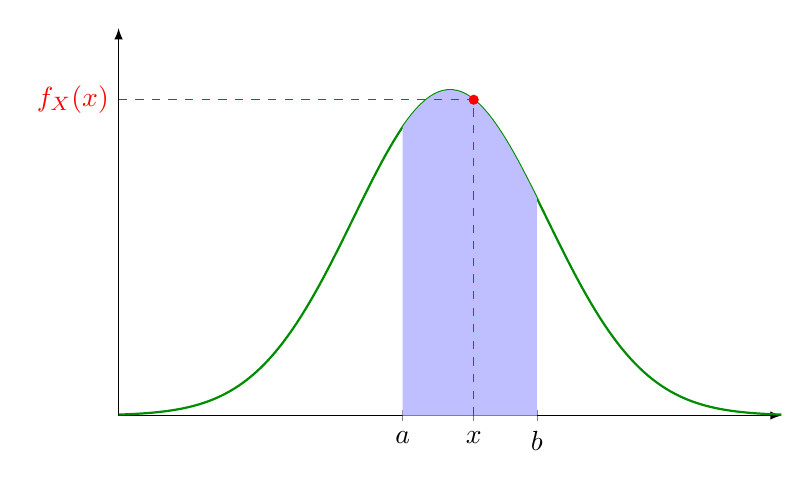
\begin{tikzpicture}
\begin{axis}[
    width=10cm, height=6.5cm,
    axis lines=left,
    xlabel={}, ylabel={},
    xtick={-0.6,0.3,1.1}, xticklabels={$a$,$x$,$b$},
    ytick=\empty,
    ymin=0, ymax=1.25,
    xmin=-4.2, xmax=4.2,
    clip=false,
    domain=-4.2:4.2, samples=150,
    axis line style={-latex},
]

% The density curve f_X(x): a bump function
\addplot[thick, green!55!black] {1.05*exp(-x^2/3)};

% Shaded region under the curve between a and b
\addplot[fill=blue!25, draw=none, domain=-0.6:1.1] {1.05*exp(-x^2/3)}
    \closedcycle;

% Dashed lookup line at x, from axis up to the curve, and across to f(x)
\draw[dashed, red] (axis cs:0.3,0) -- (axis cs:0.3,{1.05*exp(-0.09/3)});
\draw[dashed, red] (axis cs:-4.2,{1.05*exp(-0.09/3)}) -- (axis cs:0.3,{1.05*exp(-0.09/3)});
\node[red, circle, fill=red, inner sep=1.3pt] at (axis cs:0.3,{1.05*exp(-0.09/3)}) {};

% Labels
\node[red, left] at (axis cs:-4.2,{1.05*exp(-0.09/3)}) {$f_X(x)$};

% \node[anchor=south west, align=left, font=\small]
%     at (axis cs:1.8,0.55)
%     {$P(a<X<b)=\displaystyle\int_a^b f_X(x)\,dx$\\[2pt] $\;=F_X(b)-F_X(a)$};

\end{axis}
\end{tikzpicture}
\end{document}
